%\documentclass[spanish]{beamer}
\documentclass{beamer}
\usepackage{pgf,pgfpages}
%\pgfpagesuselayout{4 on 1}[letterpaper,landscape,border shrink=0.5in]
\usepackage{algorithm,algorithmic}
%\usepackage{algorithm,algorithmicx}
%\usepackage[noend]{algpseudocode}
\usepackage{listings}
\lstset{basicstyle=\ttfamily,
	showstringspaces=false,
	commentstyle=\color{red},
	literate={á}{{\'a}}1
	{ã}{{\~a}}1
	{é}{{\'e}}1
	{É}{{\'E}}1
	{ó}{{\'o}}1
	{í}{{\'i}}1
	{ñ}{{\~n}}1
	{¡}{{!`}}1
	{¿}{{?`}}1
	{ú}{{\'u}}1
	{Í}{{\'I}}1
	{Ó}{{\'O}}1
}

\usepackage{beamerthemesplit}
\usepackage{color}
\usepackage[utf8]{inputenc}
\usepackage[spanish]{babel}
%\usepackage[latin1]{inputenc}
%\usepackage[pdftex]{graphicx}
%\usepackage{algorithm}
%\usepackage{algorithmic-C}
%\usepackage{algorithmic}
\usepackage{amsthm}
\usepackage{multicol}
\usepackage{multirow}
\usepackage{fancyvrb,relsize}
\usepackage{hhline}
\usepackage{tikz}
\usetikzlibrary{trees, shapes, calc}
\newcommand{\inputTikZ}[2]{%
	\scalebox{#1}{\input{#2}}
}

\usetheme{Warsaw} %Gueno
%\usetheme{Darmstadt} %OK!
% \usetheme{Frankfurt} %OK!
%\usetheme{Goettingen}
%\usetheme{Dresden}
%\usetheme{JuanLesPins} %OK!!
%\usetheme{Marburg}
%\usetheme{Montpellier}
%\usetheme{Rochester} %sobrio
%\usetheme{Singapore}
%\usetheme{Szeged}

%\usecolortheme{albatross}
%\usecolortheme{seahorse}
%\usecolortheme{beetle}
%\usecolortheme{crane}
%\usecolortheme{dolphin}
%\usecolortheme{dove}
%\usecolortheme{fly}
%\usecolortheme{lily} %Gueno
\usecolortheme{orchid}%Gueno
%\usecolortheme{rose}
%\usecolortheme{seagull}
%\usecolortheme{whale}


\DefineVerbatimEnvironment%
      {VerbatimNN}%
      {Verbatim}%
      {fontsize=\relsize{-1}}
\DefineVerbatimEnvironment%
      {VerbatimNNN}%
      {Verbatim}%
      {fontsize=\relsize{-2}}

\DefineVerbatimEnvironment%
      {VerbatimPseudo}%
      {Verbatim}%
      {numbers=left, fontsize=\relsize{-1}}
\DefineVerbatimEnvironment%
      {VerbatimPseudoReduced}%
      {Verbatim}%
      {numbers=left, fontsize=\relsize{-2}}
\DefineVerbatimEnvironment%
      {VerbatimPseudoReduced2}%
      {Verbatim}%
      {numbers=left, fontsize=\relsize{-3}}
\DefineVerbatimEnvironment%
      {VerbatimC}%
      {Verbatim}%
      {commandchars=@ªº, numbers=left, fontsize=\relsize{-1}}
\DefineVerbatimEnvironment%
      {VerbatimReducedC}%
      {Verbatim}%
      {commandchars=@ªº, numbers=left, fontsize=\relsize{-2}}
\DefineVerbatimEnvironment%
      {VerbatimReduced2C}%
      {Verbatim}%
      {commandchars=@ªº, numbers=left, fontsize=\relsize{-3}}



%\AtBeginSubsection[]
%{
% \begin{frame}
% \frametitle{Sinopsis}
% Aqui decides: cada seccion y subseccion:
% \tableofcontents[currentsection,currentsubsection]
 %O solamente la seccion (Solo uno de ellos)
%\tableofcontents[currentsection]
% \end{frame}
%}

% Si quieres que todo por default aparezca de poco en poco
% descomenta esta linea
%\beamerdefaultoverlayspecification{<+->}

\setbeamertemplate{footline}{\hfill\insertframenumber/\inserttotalframenumber}
\setbeamertemplate{navigation symbols}{}

\setbeamercovered{transparent}

\title{ELO320 - Estructuras de Datos y Algoritmos\\Teoría de Grafos\\{\small BFS - DFS - Ordenamiento Topológico}}
%\subtitle{Ingeniería Civil Telemática UTFSM}
\author{Dr. Nicolás Gálvez R.\\{\small nicolas.galvez@usm.cl}}
\institute{Ing. Civil Telemática - Departamento de Electrónica}
\titlegraphic{
\includegraphics[scale=.18]{images/logoutfsm}}
\date{1er Semestre 2022}

\begin{document}

\frame{\titlepage}

%\section*{Sinopsis}
%\frame{  \frametitle{Sinopsis}\tableofcontents[pausesections]}
%
%

\section{Teoría de Grafos}
\begin{frame}[fragile]
 \frametitle{¿Qué es un Grafo?}\small
Es un TDA, que representa a un \textit{conjunto de objetos} los cuales pueden estar conectados mediante \textit{enlaces}. 

\begin{center}
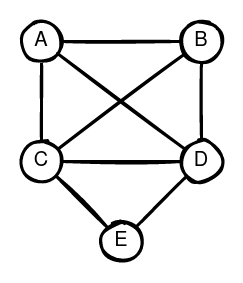
\includegraphics[width=0.3\linewidth]{images/graphs/graph-undirected}
\end{center}

Los grafos son fácilmente graficables, y en estos los objetos representados por nodos, llamados \textbf{vértices}, están interconectados enlaces denominados \textbf{aritstas}.
\end{frame}

\begin{frame}[fragile]
 \frametitle{Aplicaciones}
\begin{center}
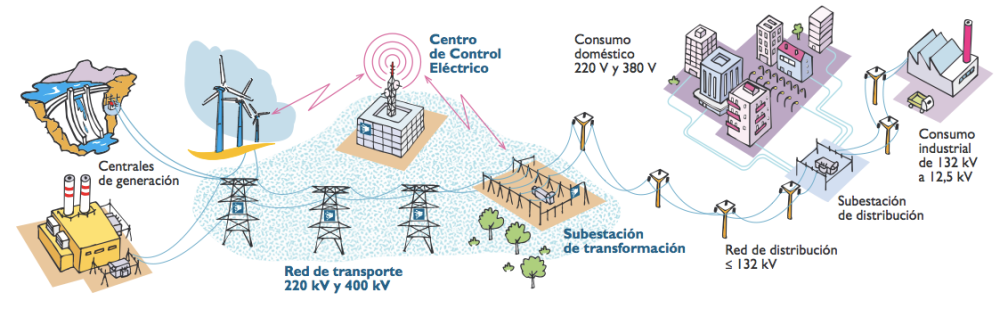
\includegraphics[width=0.95\linewidth]{images/graphs/redelec}

Redes Eléctricas
\end{center}
\end{frame}

\begin{frame}[fragile]
 \frametitle{Aplicaciones}
\begin{center}
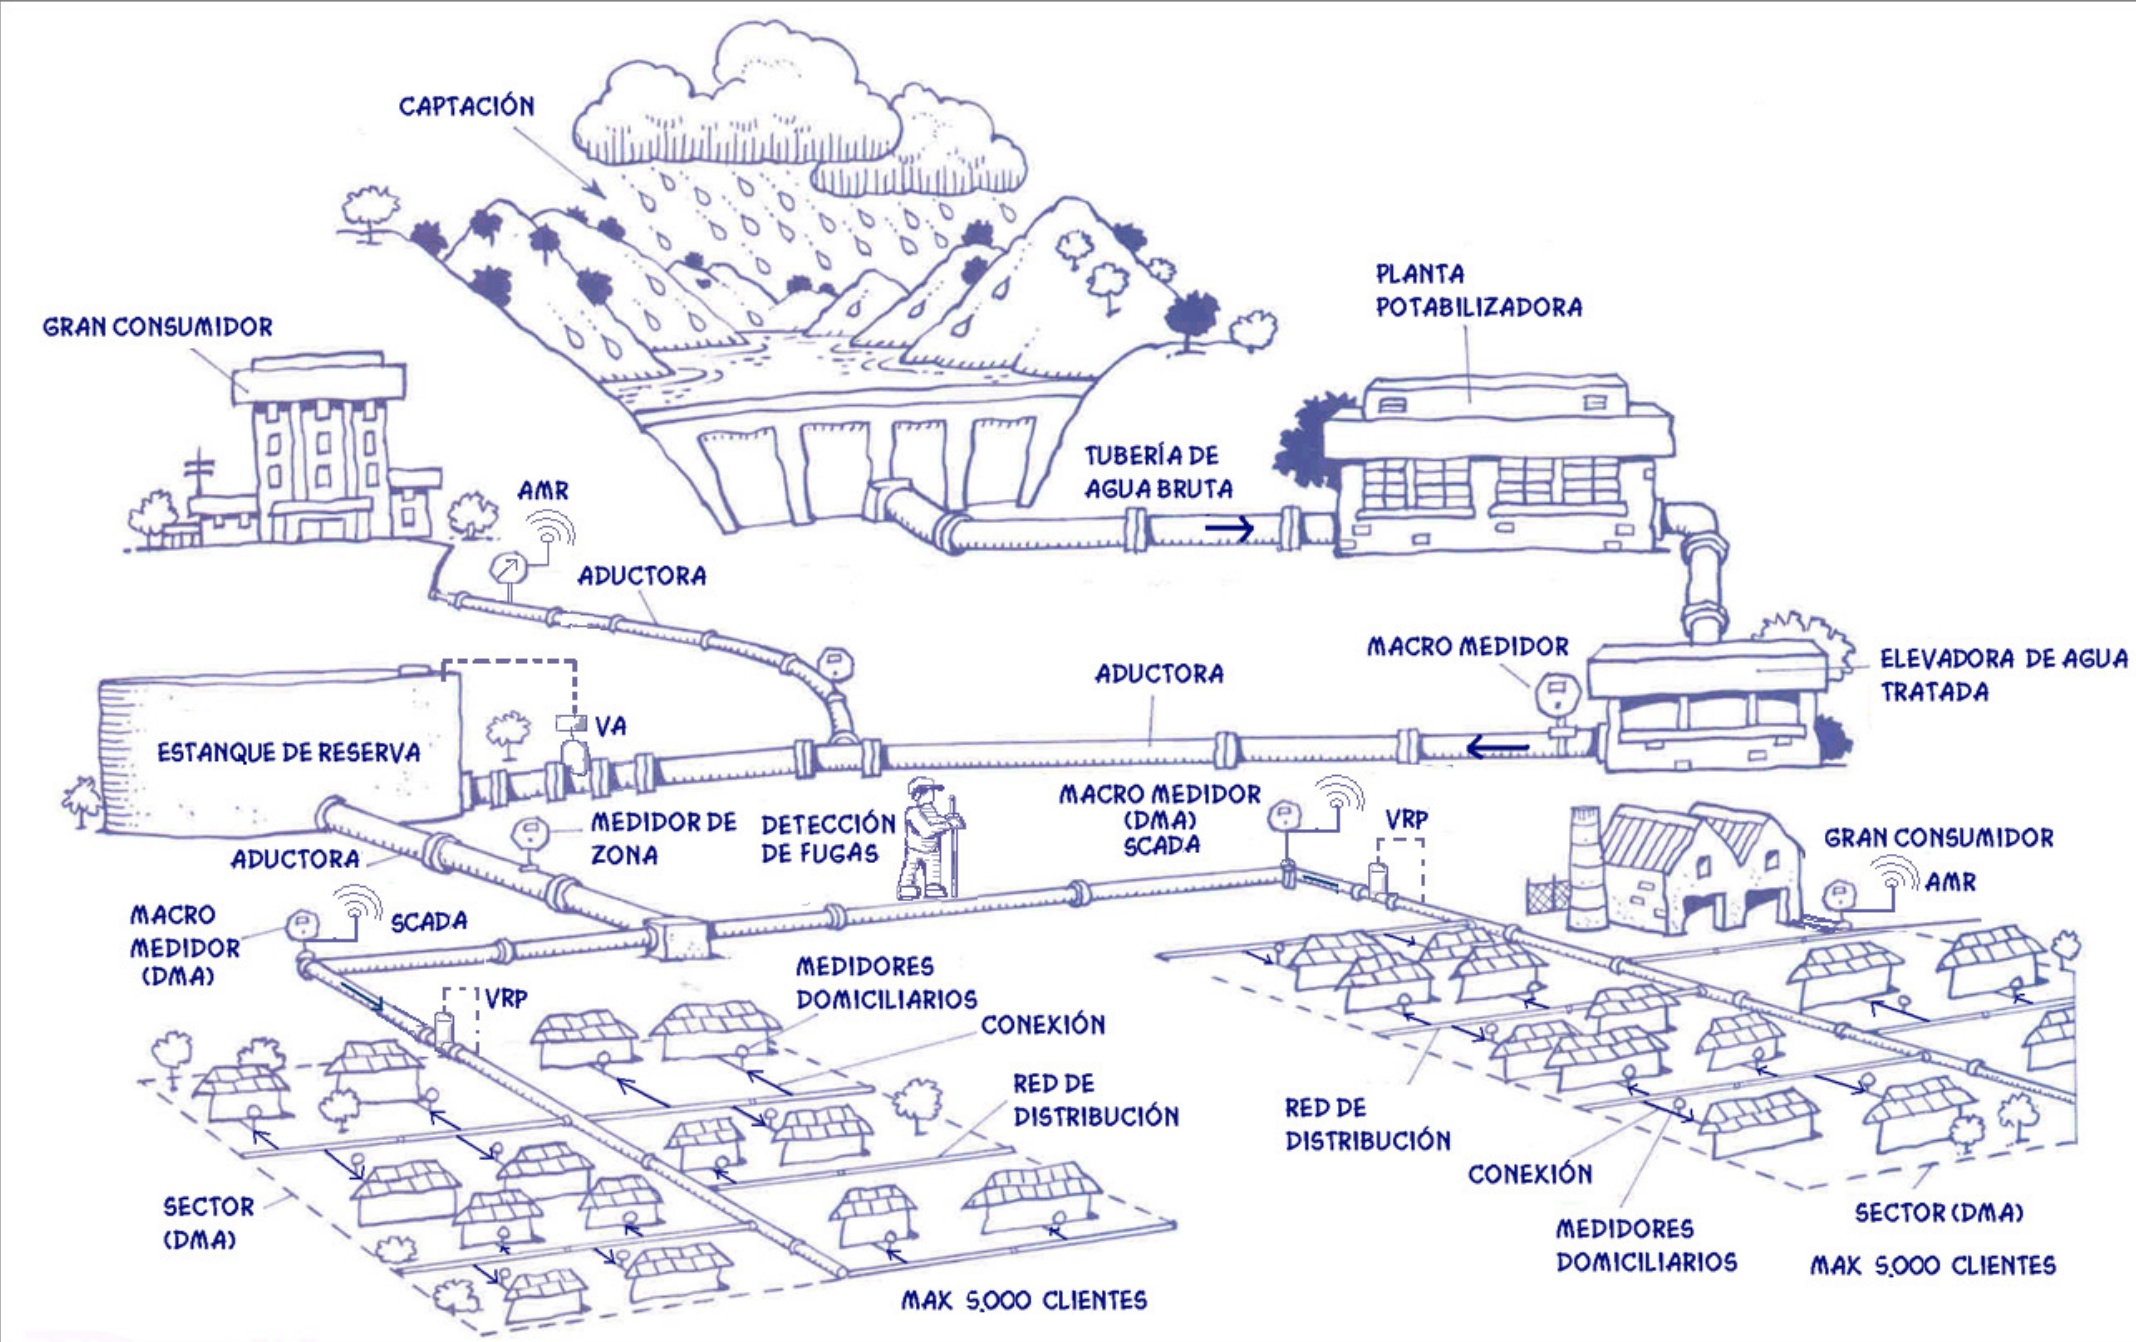
\includegraphics[width=0.95\linewidth]{images/graphs/redagua}

Redes de Agua Potable
\end{center}
\end{frame}

\begin{frame}[fragile]
 \frametitle{Aplicaciones}
\begin{center}
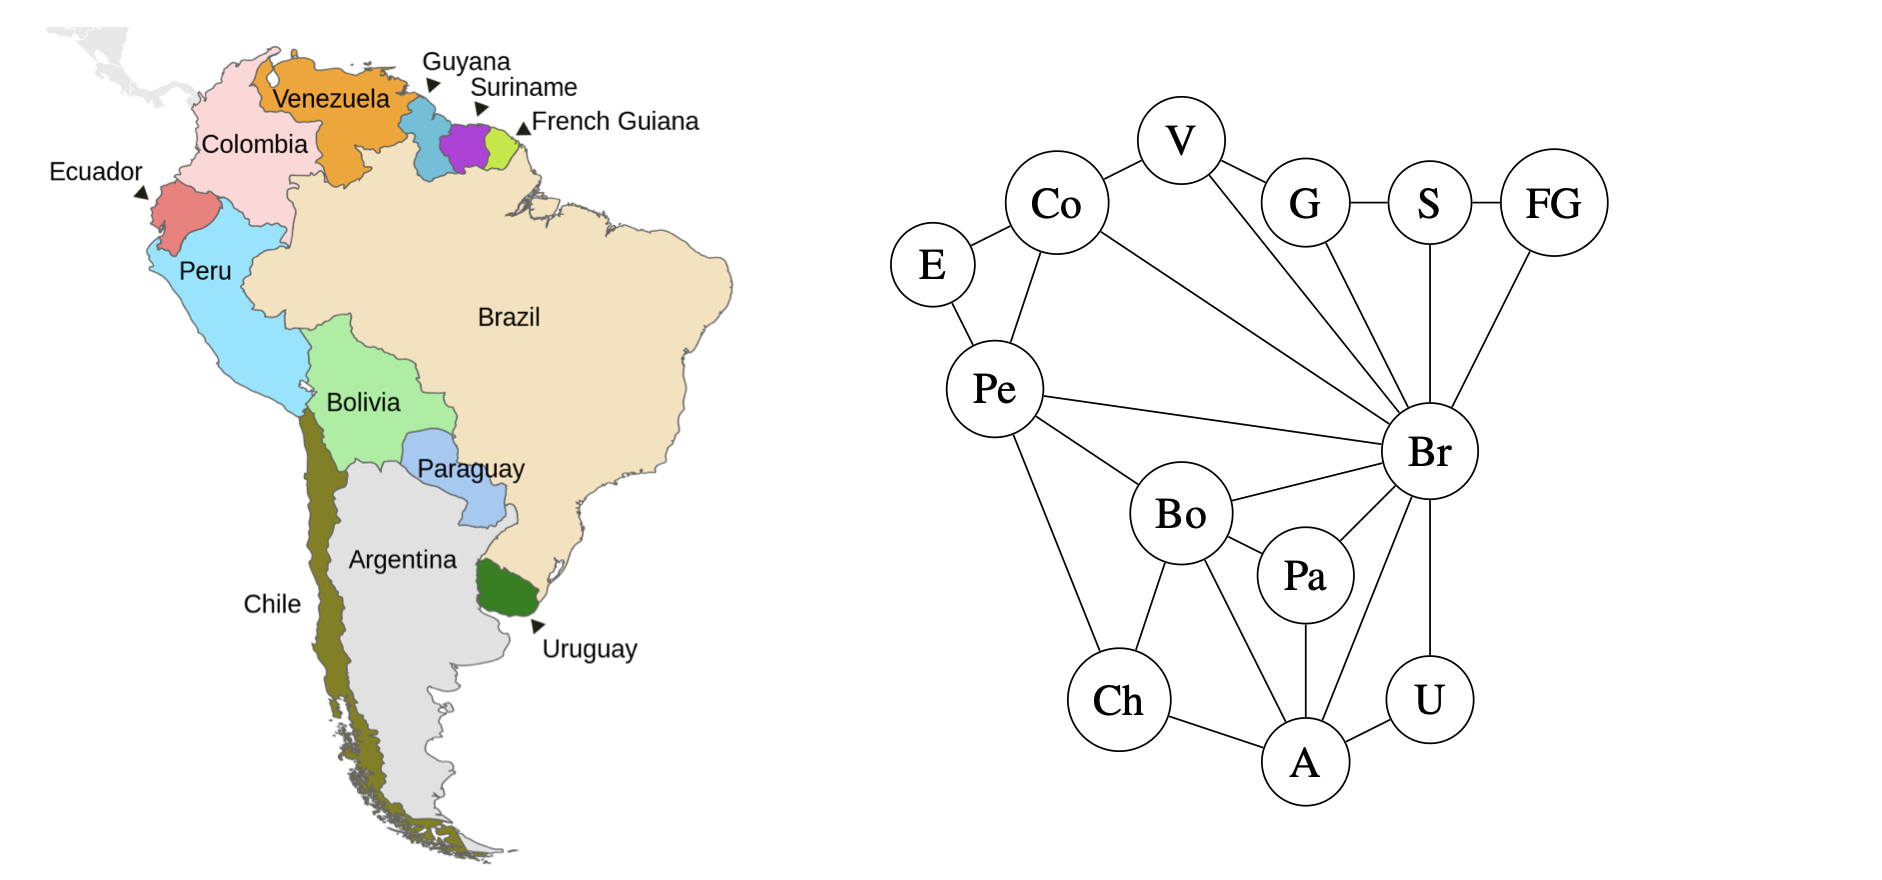
\includegraphics[width=0.95\linewidth]{images/graphs/southamerica}

Coloreo de Mapas
\end{center}
\end{frame}


\section{Formalización y Definiciones}
\begin{frame}[fragile]
 \frametitle{Formalización de Grafos}\small
Un grafo se define como una tupla $\mathcal{G} = (\mathcal{V}, \mathcal{A})$, en donde:
\begin{itemize}
\item $\mathcal{V}$: Es el conjunto de \textbf{vértices} o \textbf{nodos},
\item $\mathcal{A} = \{ (x,y)\ |\ (x,y) \in \mathcal{V}^2 \land x \neq y \}$: Es el conjunto de \textbf{aristas} o \textbf{enlaces}.
\end{itemize}

\begin{center}
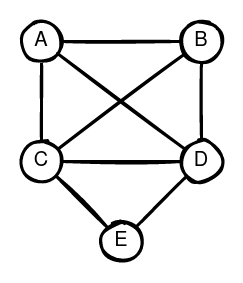
\includegraphics[width=0.3\linewidth]{images/graphs/graph-undirected}
\end{center}

Note que un arco $(x,y) \in \mathcal{A}$ conecta a dos nodos $x \in \mathcal{V} $ e $y \in \mathcal{V}$.
\end{frame}

\begin{frame}[fragile]
 \frametitle{Formalización de Grafos}
\small
Un grafo se define como una tupla $\mathcal{G} = (\mathcal{V}, \mathcal{A})$, en donde:
\begin{itemize}
\item $\mathcal{V} = \{A,B,C,D,E\}$.
\item $\mathcal{A} = \{(A,B), (A,C), (A,D), (B,C), (B,D), (C,D), (C,E), (D,E) \}$.
\end{itemize}
\begin{center}
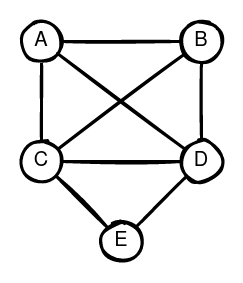
\includegraphics[width=0.3\linewidth]{images/graphs/graph-undirected}
\end{center}
\end{frame}


\begin{frame}[fragile]
 \frametitle{Conceptos}\small
\begin{itemize}
\item Grafo No Dirigido: Enlaces sin dirección (o con todas las direcciones)
\begin{center}
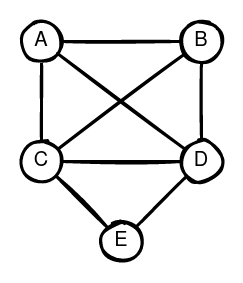
\includegraphics[width=0.275\linewidth]{images/graphs/graph-undirected}
\end{center}
\item Grafo Dirigido: Enlaces con una dirección específica.
\begin{center}
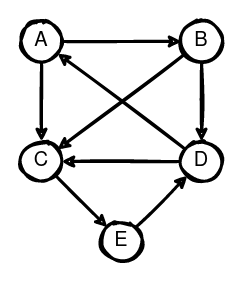
\includegraphics[width=0.275\linewidth]{images/graphs/graph-directed}
\end{center}
\end{itemize}
\end{frame}


\begin{frame}[fragile]
 \frametitle{Conceptos}\small
\begin{itemize}
\item Grafo no Ponderado: Enlaces no poseen valor o son equivalentes.
\begin{center}
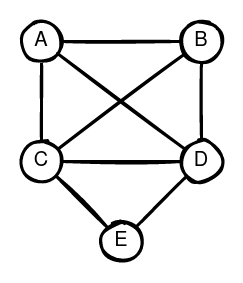
\includegraphics[width=0.275\linewidth]{images/graphs/graph-undirected}
\end{center}
\item Grafo Ponderado: Enlaces poseen diferentes pesos o valores. 
\begin{center}
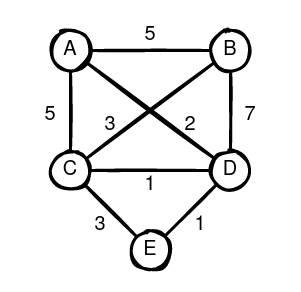
\includegraphics[width=0.275\linewidth]{images/graphs/graph-weighted}
\end{center}
\end{itemize}
\end{frame}

\begin{frame}[fragile]
 \frametitle{Conceptos}\small
\begin{itemize}
\item Nodos Adyacentes: Nodos que se separan sólo por una arista.
\begin{center}
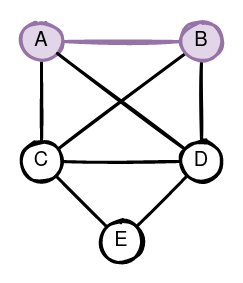
\includegraphics[width=0.3\linewidth]{images/graphs/graph-adjacent}
\end{center}
\item Vecindario: Todos los nodos adyacentes respecto a un vértice.
\begin{center}
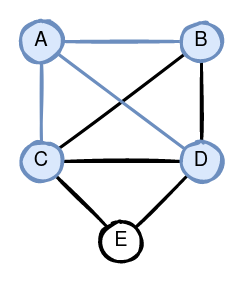
\includegraphics[width=0.3\linewidth]{images/graphs/graph-neighbourhood}
\end{center}
\end{itemize}
\end{frame}


\begin{frame}[fragile]
 \frametitle{Conceptos}\small
\begin{itemize}
\item Cadena: Secuencia de enlaces tal que cada arista tiene exactamente un vértice en común con la arista previa.
\begin{center}
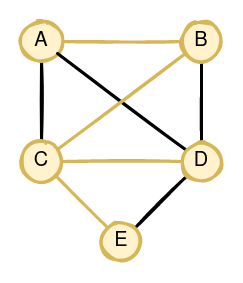
\includegraphics[width=0.26\linewidth]{images/graphs/graph-chain}
\end{center}
\item Camino: Secuencia de enlaces tal que cada vértice terminal de una arísta es idéntica al vértice inicial de la siguiente. 
\begin{center}
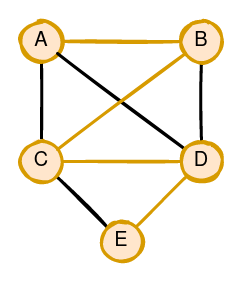
\includegraphics[width=0.26\linewidth]{images/graphs/graph-path}
\end{center}
\end{itemize}
\end{frame}

\begin{frame}[fragile]
 \frametitle{Conceptos}\small
\begin{itemize}
\item Ciclo: Camino en el que el vértice terminal de la última arísta es idéntico al vertice inicial de la primera.
\begin{center}
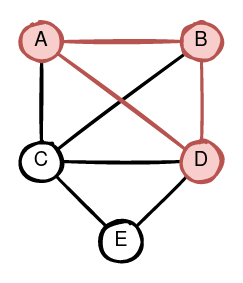
\includegraphics[width=0.26\linewidth]{images/graphs/graph-cycle}
\end{center}
\item Árbol de Expansión: Cadena de $(n-1)$ arcos que conecta toda la red y no contiene ciclos.
\begin{center}
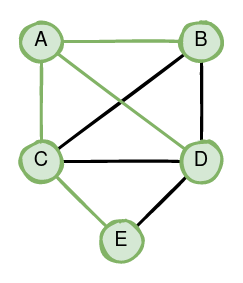
\includegraphics[width=0.26\linewidth]{images/graphs/graph-spanning-tree}
\end{center}
\end{itemize}
\end{frame}

\begin{frame}[fragile]
 \frametitle{Representación: Lista de Adyacencia}\small
\begin{itemize}
\item Utilizados para grafos escasos (sparce) $\rightarrow |\mathcal{A}| <<< |\mathcal{V}|^2$.
\item Arreglo de listas donde se almacenan los enlaces involucrados. 
\item Grafo No Dirigido:
\begin{center}
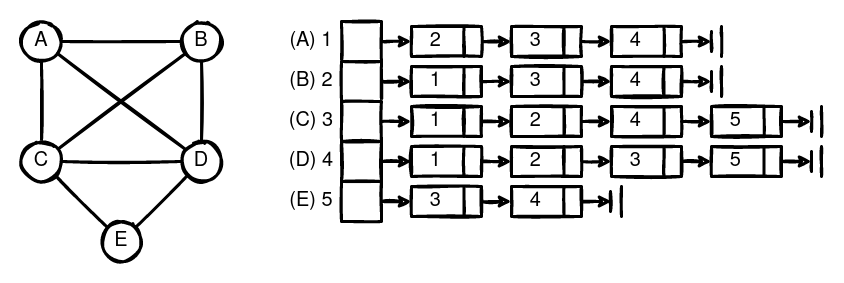
\includegraphics[width=0.95\linewidth]{images/graphs/graph-adjacent-list-undirected}
\end{center}
%\item Memoria: $\Theta(\mathcal{V}+\mathcal{A})$.
%\item Añadir Vértice: $\mathcal{O}(1)$.
%\item Añadir Arista: $\mathcal{O}(1)$.
%\item Eliminar Vértice: $\mathcal{O}(\mathcal{V}+\mathcal{A})$
%\item Buscar Arista: $\mathcal{O}(\mathcal{V})$
\end{itemize}
\end{frame}


\begin{frame}[fragile]
 \frametitle{Representación: Lista de Adyacencia}\small
\begin{itemize}
\item Grafo Dirigido:
\begin{center}
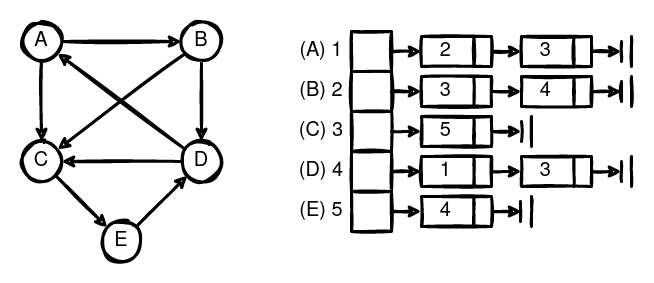
\includegraphics[width=0.75\linewidth]{images/graphs/graph-adjacent-list-directed}
\end{center}
\item Memoria: $\Theta(|\mathcal{V}|+|\mathcal{A}|)$.
\item Añadir Vértice: $\mathcal{O}(1)$.
\item Añadir Arista: $\mathcal{O}(1)$.
\item Eliminar Vértice: $\mathcal{O}(|\mathcal{V}|+|\mathcal{A}|)$.
\item Eliminar Arista: $\mathcal{O}(|\mathcal{A}|)$.
\item Buscar Arista: $\mathcal{O}(|\mathcal{V}|)$.
\end{itemize}

\end{frame}


\begin{frame}[fragile]
 \frametitle{Representación: Matriz de Adyacencia}\small
\begin{itemize}
\item Utilizados para grafos densos, o cuando se necesita acceso rápido a los enlaces.
\item Arreglo binario bidimensional: $A[i][j]$ indica si existe un enlace entre el nodo $i$ y el nodo $j$. 
\item Grafo No Dirigido: Matriz Simétrica.
\begin{center}
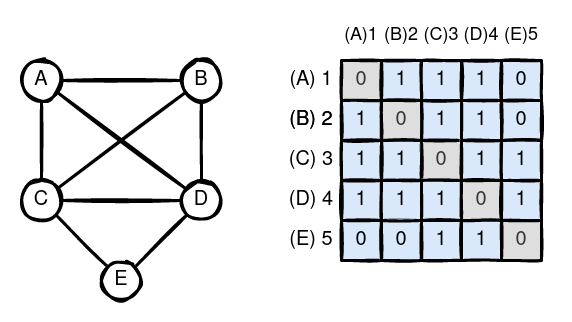
\includegraphics[width=0.75\linewidth]{images/graphs/graph-adjacent-matrix-undirected}
\end{center}
%\item Memoria: $\Theta(\mathcal{V}+\mathcal{A})$.
%\item Añadir Vértice: $\mathcal{O}(1)$.
%\item Añadir Arista: $\mathcal{O}(1)$.
%\item Eliminar Vértice: $\mathcal{O}(\mathcal{V}+\mathcal{A})$
%\item Buscar Arista: $\mathcal{O}(\mathcal{V})$
\end{itemize}

\end{frame}

\begin{frame}[fragile]
 \frametitle{Representación: Matriz de Adyacencia}\small
\begin{itemize}
\item Grafo Dirigido: Matriz Asimétrica.
\begin{center}
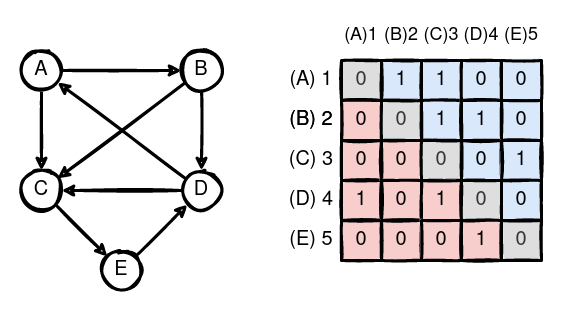
\includegraphics[width=0.75\linewidth]{images/graphs/graph-adjacent-matrix-directed}
\end{center}
\item Memoria: $\Theta(|\mathcal{V}|^2)$.
\item Añadir Vértice: $\mathcal{O}(|\mathcal{V}|^2)$.
\item Añadir Arista: $\mathcal{O}(1)$.
\item Eliminar Vértice: $\mathcal{O}(|\mathcal{V}|^2)$
\item Eliminar Arista: $\mathcal{O}(1)$.
\item Buscar Arista: $\mathcal{O}(1)$
\end{itemize}

\end{frame}

\section{Recorrido en Grafos: Búsqueda.}
\begin{frame}[fragile]
 \frametitle{Búsqueda en Grafos}\small
\begin{itemize}
\item \textbf{Problema de búsqueda}: verificar la existencia o no existencia de un elemento en un espacio determinado (espacio de búsqueda).
\item En grafos: \textbf{Especificar un orden para encontrar un elemento a través de los componentes de un grafo}.
\item En los problemas de búsqueda, existen dos criterios clásicos, no excluyentes, que tienen directo impacto en la efectividad de la búsqueda:
\begin{itemize}
\item Exploración: Diversificar la zona cubierta del espacio de búsqueda para encontrar la solución.
\item Explotación: Intensificar la busqueda en la zona ya descubierta. 
\end{itemize}
\item Los algortimo de búsqueda, en diversas áreas, combinan en distintos rangos estos criterios. 
  
\end{itemize}
\end{frame}

\begin{frame}[fragile]
 \frametitle{Breadth-first Search (BFS)}\small
\begin{itemize}
\item Búsqueda en Anchura o BFS, es un algoritmo de busqueda sin información que encuentra, desde un nodo, el mínimo recorrido (en arcos), hacia el resto de los nodos.
\item Ponderá la exploración de vecinos por sobre la explotación de ramas.
\item Tal como en árboles, utiliza una cola como TDA auxiliar.
\item Resultado: árbol de expansión BFS.
\end{itemize}
\end{frame}

\begin{frame}[fragile]
 \frametitle{Breadth-first Search (BFS) no dirigido}\small
\begin{center}
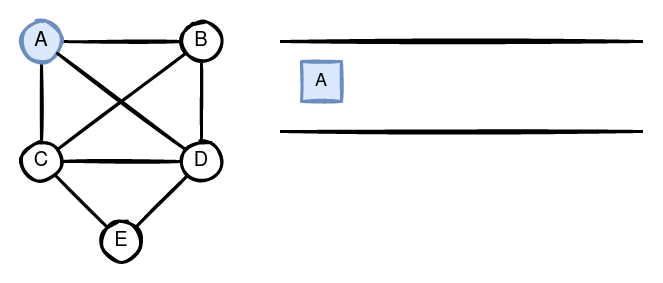
\includegraphics[width=0.8\linewidth]{images/graphs/graph-bfs-undirected-1}
\end{center}
\end{frame}

\begin{frame}[fragile]
 \frametitle{Breadth-first Search (BFS) no dirigido}\small
\begin{center}
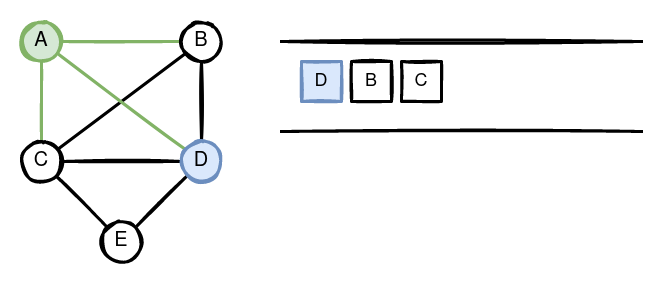
\includegraphics[width=0.8\linewidth]{images/graphs/graph-bfs-undirected-2}
\end{center}
\end{frame}

\begin{frame}[fragile]
 \frametitle{Breadth-first Search (BFS) no dirigido}\small
\begin{center}
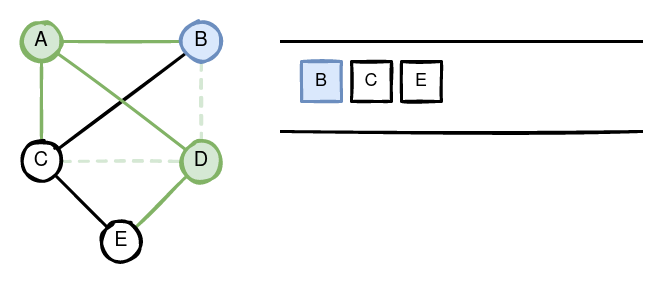
\includegraphics[width=0.8\linewidth]{images/graphs/graph-bfs-undirected-3}
\end{center}
\end{frame}

\begin{frame}[fragile]
 \frametitle{Breadth-first Search (BFS) no dirigido}\small
\begin{center}
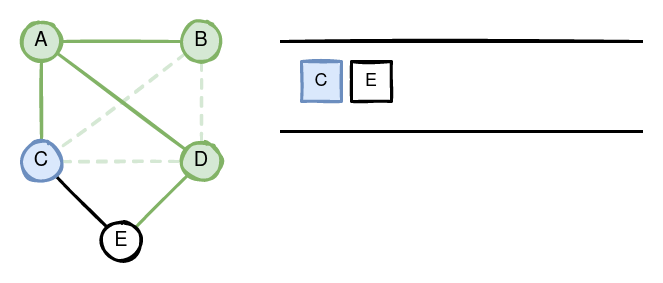
\includegraphics[width=0.8\linewidth]{images/graphs/graph-bfs-undirected-4}
\end{center}
\end{frame}

\begin{frame}[fragile]
 \frametitle{Breadth-first Search (BFS) no dirigido}\small
\begin{center}
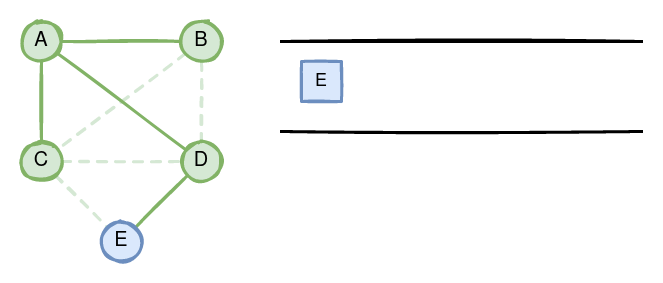
\includegraphics[width=0.8\linewidth]{images/graphs/graph-bfs-undirected-5}
\end{center}
\end{frame}

\begin{frame}[fragile]
 \frametitle{Breadth-first Search (BFS) no dirigido}\small
\begin{center}
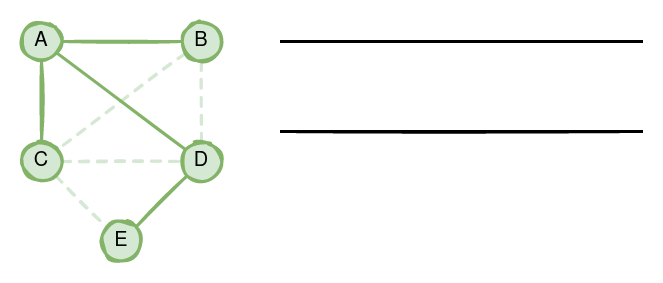
\includegraphics[width=0.8\linewidth]{images/graphs/graph-bfs-undirected-6}
\end{center}
\end{frame}

\begin{frame}[fragile]
 \frametitle{Breadth-first Search (BFS) dirigido}\small
\begin{center}
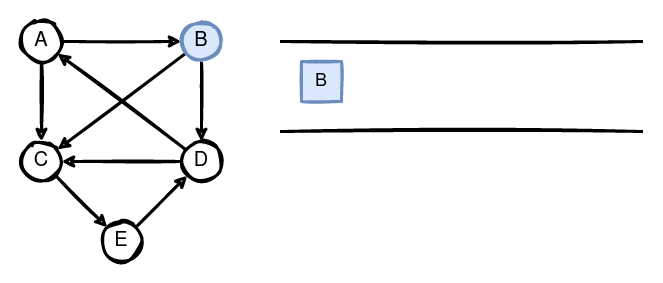
\includegraphics[width=0.8\linewidth]{images/graphs/graph-bfs-directed-1}
\end{center}
\end{frame}

\begin{frame}[fragile]
 \frametitle{Breadth-first Search (BFS) dirigido}\small
\begin{center}
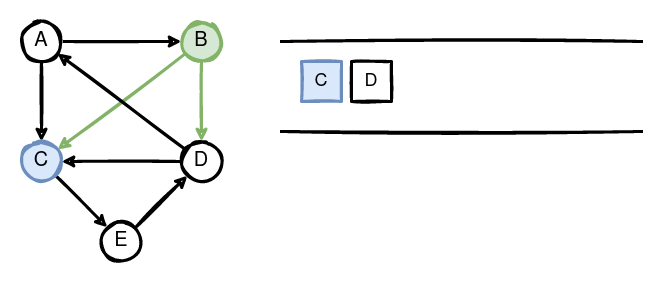
\includegraphics[width=0.8\linewidth]{images/graphs/graph-bfs-directed-2}
\end{center}
\end{frame}

\begin{frame}[fragile]
 \frametitle{Breadth-first Search (BFS) dirigido}\small
\begin{center}
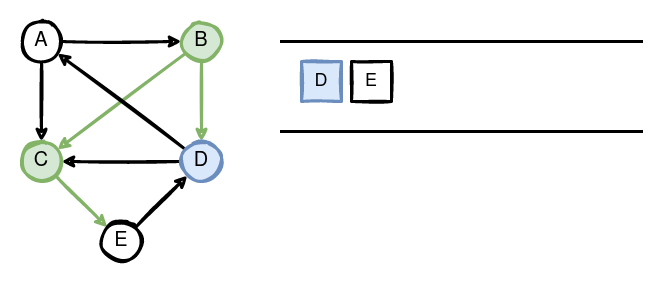
\includegraphics[width=0.8\linewidth]{images/graphs/graph-bfs-directed-3}
\end{center}
\end{frame}

\begin{frame}[fragile]
 \frametitle{Breadth-first Search (BFS) dirigido}\small
\begin{center}
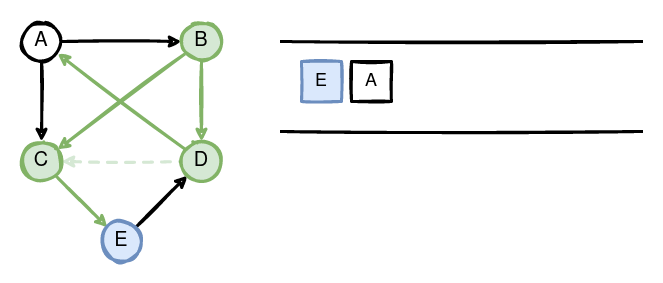
\includegraphics[width=0.8\linewidth]{images/graphs/graph-bfs-directed-4}
\end{center}
\end{frame}

\begin{frame}[fragile]
 \frametitle{Breadth-first Search (BFS) dirigido}\small
\begin{center}
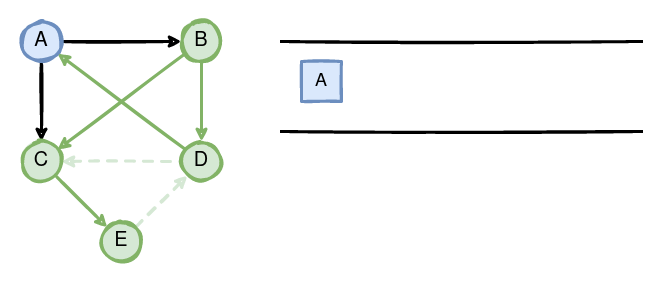
\includegraphics[width=0.8\linewidth]{images/graphs/graph-bfs-directed-5}
\end{center}
\end{frame}

\begin{frame}[fragile]
 \frametitle{Breadth-first Search (BFS) dirigido}\small
\begin{center}
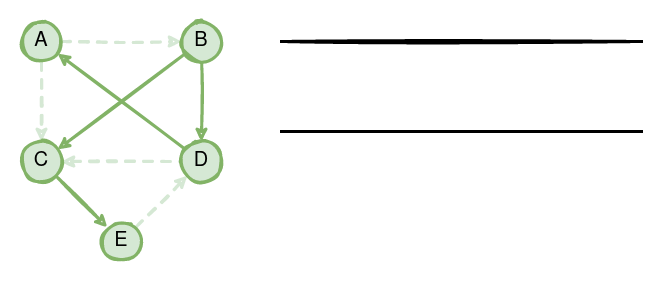
\includegraphics[width=0.8\linewidth]{images/graphs/graph-bfs-directed-6}
\end{center}
\end{frame}

\begin{frame}[fragile]
 \frametitle{Breadth-first Search (BFS) Árbol Binario}\small
\begin{center}
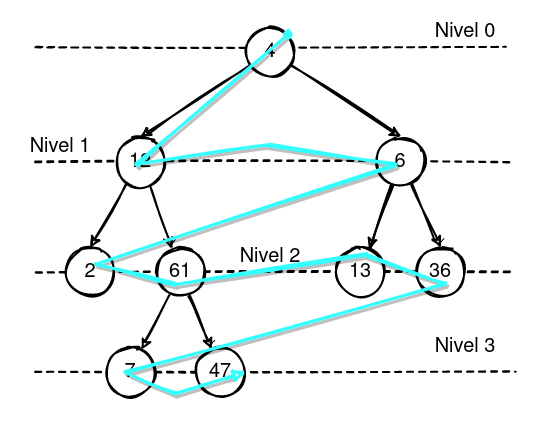
\includegraphics[width=0.8\linewidth]{images/breadthsearch}
\end{center}
\end{frame}

\begin{frame}[fragile]
 \frametitle{Depth-first Search (DFS)}\small
\begin{itemize}
\item Búsqueda en Profundidad o DFS, es un algoritmo de busqueda sin información que encuentra, desde un nodo, las ramas más profundas (en arcos), hacia el resto de los nodos.
\item Ponderá la explotación de ramas por sobre la exploración de vecinos.
\item Utiliza una pila como TDA auxilia.   
\item Resultado: árbol de expansión DFS.
\end{itemize}
\end{frame}

\begin{frame}[fragile]
 \frametitle{Depth-first Search (DFS) no dirigido}\small
\begin{center}
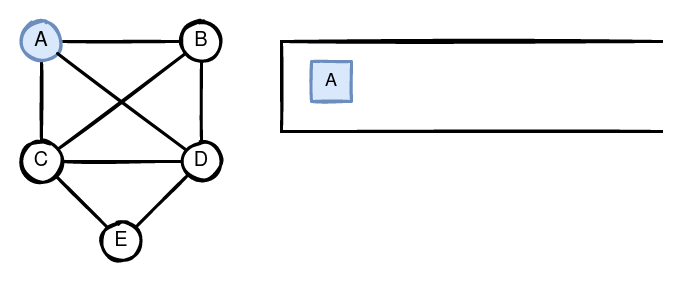
\includegraphics[width=0.8\linewidth]{images/graphs/graph-dfs-undirected-1}
\end{center}
\end{frame}

\begin{frame}[fragile]
 \frametitle{Depth-first Search (DFS) no dirigido}\small
\begin{center}
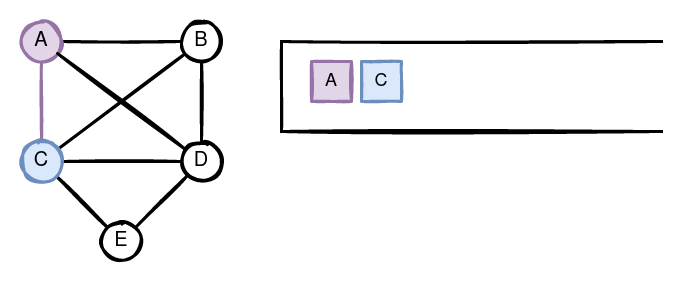
\includegraphics[width=0.8\linewidth]{images/graphs/graph-dfs-undirected-2}
\end{center}
\end{frame}

\begin{frame}[fragile]
 \frametitle{Depth-first Search (DFS) no dirigido}\small
\begin{center}
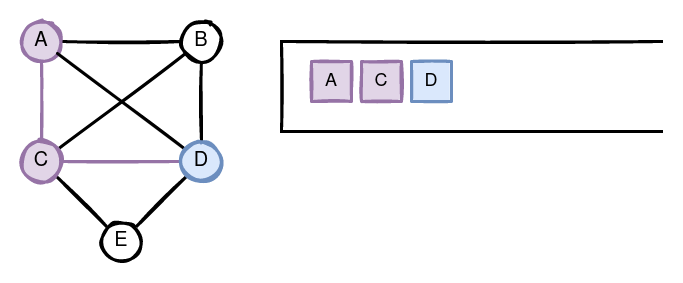
\includegraphics[width=0.8\linewidth]{images/graphs/graph-dfs-undirected-3}
\end{center}
\end{frame}

\begin{frame}[fragile]
 \frametitle{Depth-first Search (DFS) no dirigido}\small
\begin{center}
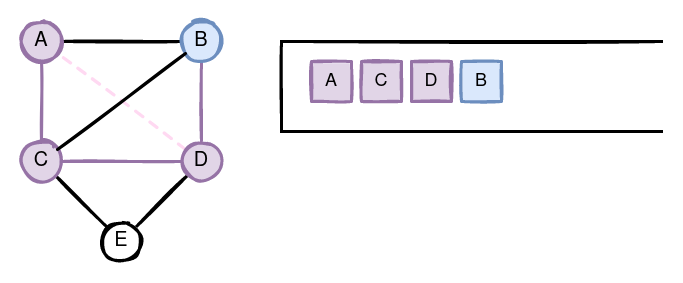
\includegraphics[width=0.8\linewidth]{images/graphs/graph-dfs-undirected-4}
\end{center}
\end{frame}

\begin{frame}[fragile]
 \frametitle{Depth-first Search (DFS) no dirigido}\small
\begin{center}
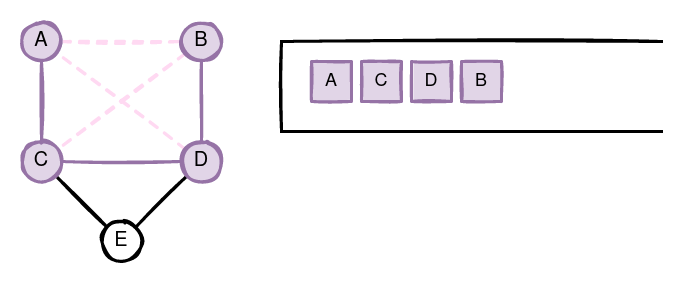
\includegraphics[width=0.8\linewidth]{images/graphs/graph-dfs-undirected-5}
\end{center}
\end{frame}

\begin{frame}[fragile]
 \frametitle{Depth-first Search (DFS) no dirigido}\small
\begin{center}
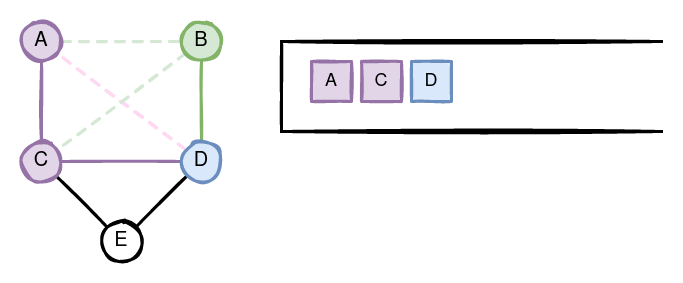
\includegraphics[width=0.8\linewidth]{images/graphs/graph-dfs-undirected-6}
\end{center}
\end{frame}

\begin{frame}[fragile]
 \frametitle{Depth-first Search (DFS) no dirigido}\small
\begin{center}
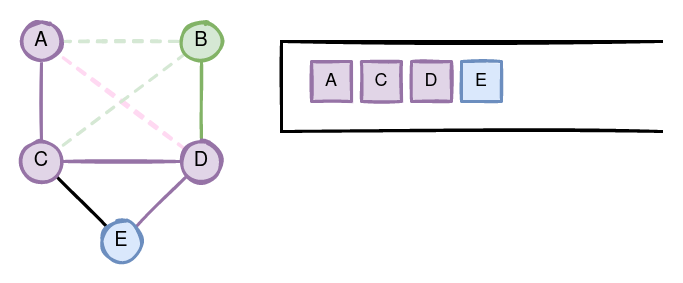
\includegraphics[width=0.8\linewidth]{images/graphs/graph-dfs-undirected-7}
\end{center}
\end{frame}

\begin{frame}[fragile]
 \frametitle{Depth-first Search (DFS) no dirigido}\small
\begin{center}
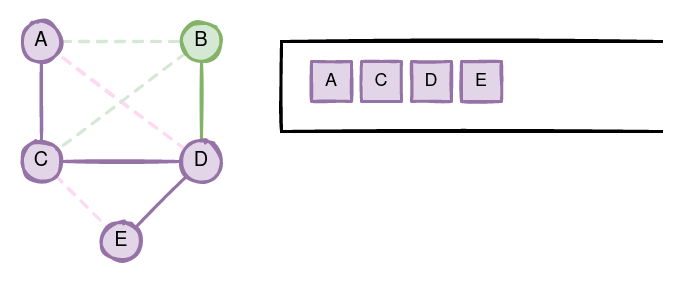
\includegraphics[width=0.8\linewidth]{images/graphs/graph-dfs-undirected-8}
\end{center}
\end{frame}

\begin{frame}[fragile]
 \frametitle{Depth-first Search (DFS) no dirigido}\small
\begin{center}
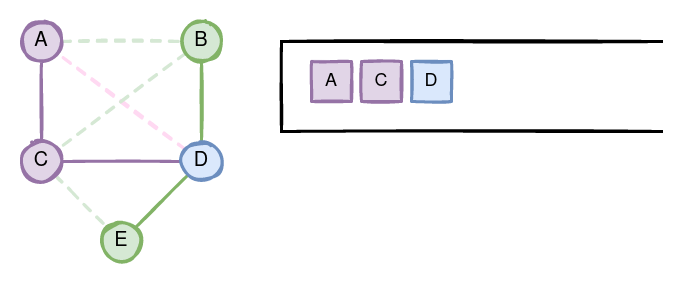
\includegraphics[width=0.8\linewidth]{images/graphs/graph-dfs-undirected-9}
\end{center}
\end{frame}

\begin{frame}[fragile]
 \frametitle{Depth-first Search (DFS) no dirigido}\small
\begin{center}
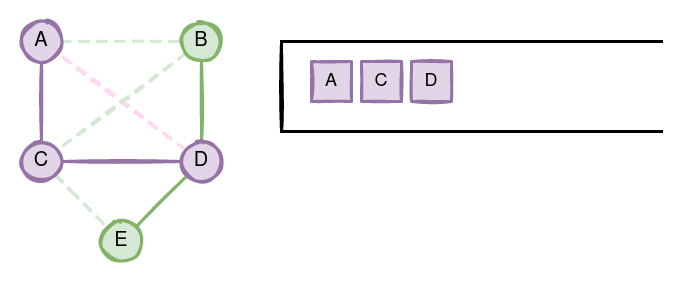
\includegraphics[width=0.8\linewidth]{images/graphs/graph-dfs-undirected-10}
\end{center}
\end{frame}

\begin{frame}[fragile]
 \frametitle{Depth-first Search (DFS) no dirigido}\small
\begin{center}
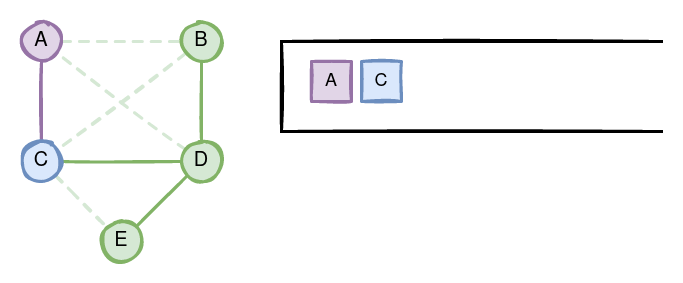
\includegraphics[width=0.8\linewidth]{images/graphs/graph-dfs-undirected-11}
\end{center}
\end{frame}

\begin{frame}[fragile]
 \frametitle{Depth-first Search (DFS) no dirigido}\small
\begin{center}
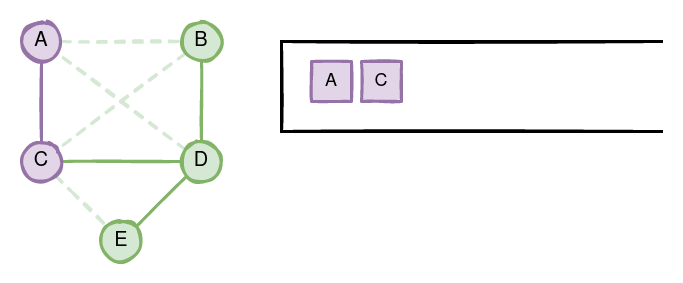
\includegraphics[width=0.8\linewidth]{images/graphs/graph-dfs-undirected-12}
\end{center}
\end{frame}

\begin{frame}[fragile]
 \frametitle{Depth-first Search (DFS) no dirigido}\small
\begin{center}
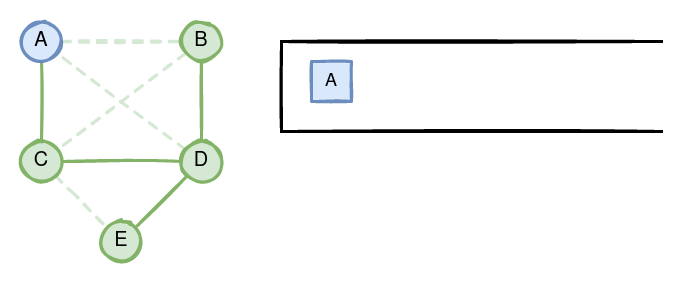
\includegraphics[width=0.8\linewidth]{images/graphs/graph-dfs-undirected-13}
\end{center}
\end{frame}

\begin{frame}[fragile]
 \frametitle{Depth-first Search (DFS) no dirigido}\small
\begin{center}
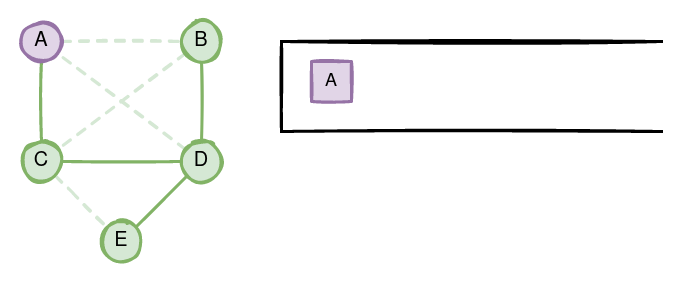
\includegraphics[width=0.8\linewidth]{images/graphs/graph-dfs-undirected-14}
\end{center}
\end{frame}

\begin{frame}[fragile]
 \frametitle{Depth-first Search (DFS) no dirigido}\small
\begin{center}
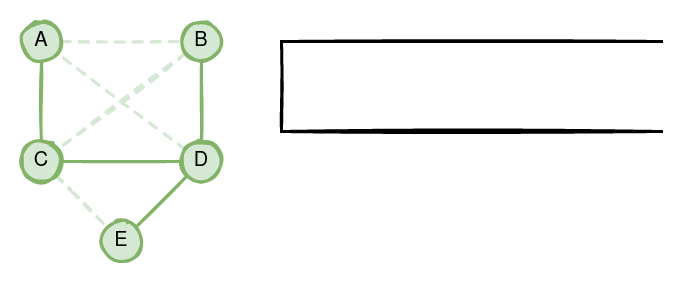
\includegraphics[width=0.8\linewidth]{images/graphs/graph-dfs-undirected-15}
\end{center}
\end{frame}

\begin{frame}[fragile]
 \frametitle{Depth-first Search (DFS) dirigido}\small
\begin{center}
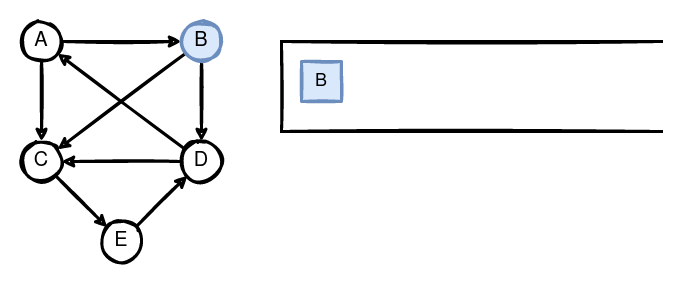
\includegraphics[width=0.8\linewidth]{images/graphs/graph-dfs-directed-1}
\end{center}
\end{frame}

\begin{frame}[fragile]
 \frametitle{Depth-first Search (DFS) dirigido}\small
\begin{center}
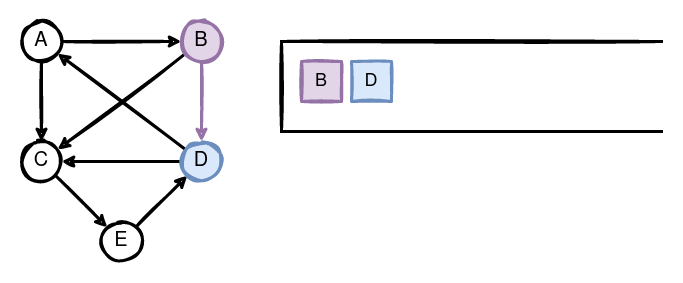
\includegraphics[width=0.8\linewidth]{images/graphs/graph-dfs-directed-2}
\end{center}
\end{frame}

\begin{frame}[fragile]
 \frametitle{Depth-first Search (DFS) dirigido}\small
\begin{center}
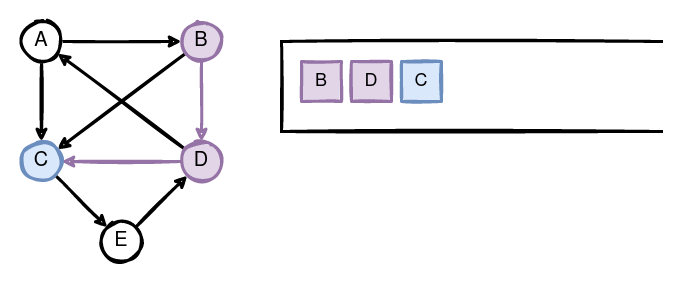
\includegraphics[width=0.8\linewidth]{images/graphs/graph-dfs-directed-3}
\end{center}
\end{frame}

\begin{frame}[fragile]
 \frametitle{Depth-first Search (DFS) dirigido}\small
\begin{center}
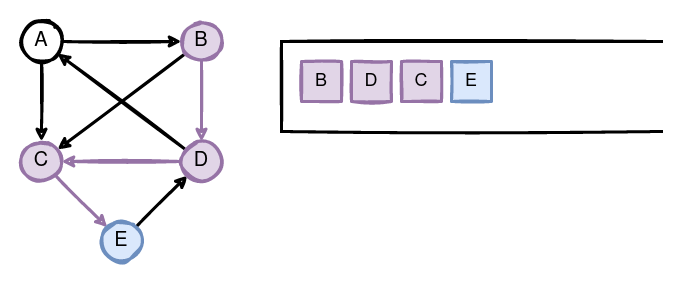
\includegraphics[width=0.8\linewidth]{images/graphs/graph-dfs-directed-4}
\end{center}
\end{frame}

\begin{frame}[fragile]
 \frametitle{Depth-first Search (DFS) dirigido}\small
\begin{center}
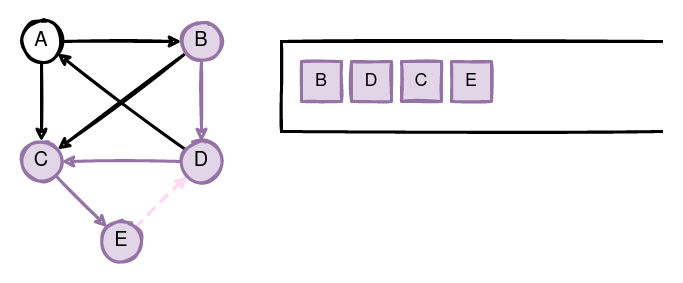
\includegraphics[width=0.8\linewidth]{images/graphs/graph-dfs-directed-5}
\end{center}
\end{frame}

\begin{frame}[fragile]
 \frametitle{Depth-first Search (DFS) dirigido}\small
\begin{center}
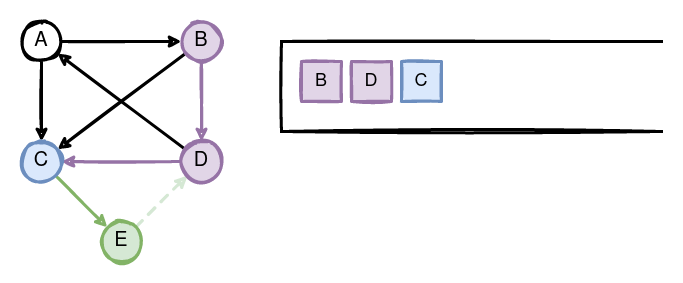
\includegraphics[width=0.8\linewidth]{images/graphs/graph-dfs-directed-6}
\end{center}
\end{frame}

\begin{frame}[fragile]
 \frametitle{Depth-first Search (DFS) dirigido}\small
\begin{center}
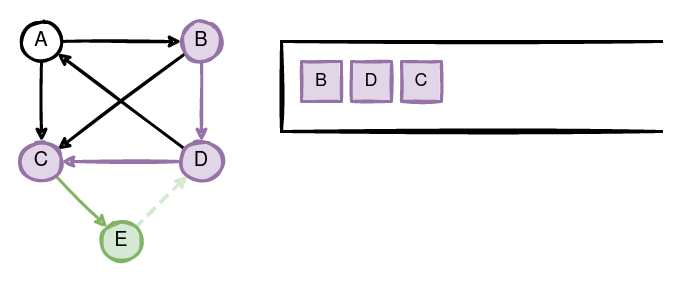
\includegraphics[width=0.8\linewidth]{images/graphs/graph-dfs-directed-7}
\end{center}
\end{frame}

\begin{frame}[fragile]
 \frametitle{Depth-first Search (DFS) dirigido}\small
\begin{center}
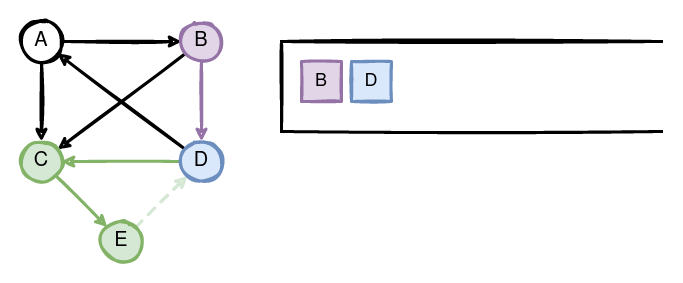
\includegraphics[width=0.8\linewidth]{images/graphs/graph-dfs-directed-8}
\end{center}
\end{frame}

\begin{frame}[fragile]
 \frametitle{Depth-first Search (DFS) dirigido}\small
\begin{center}
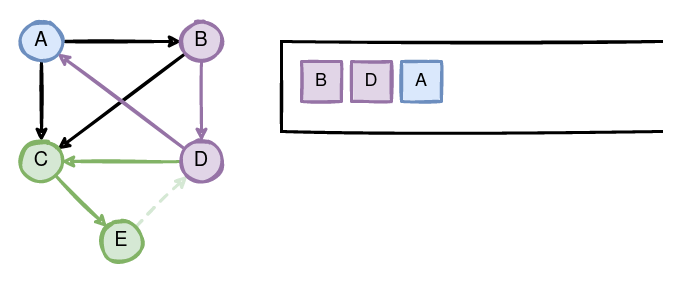
\includegraphics[width=0.8\linewidth]{images/graphs/graph-dfs-directed-9}
\end{center}
\end{frame}

\begin{frame}[fragile]
 \frametitle{Depth-first Search (DFS) dirigido}\small
\begin{center}
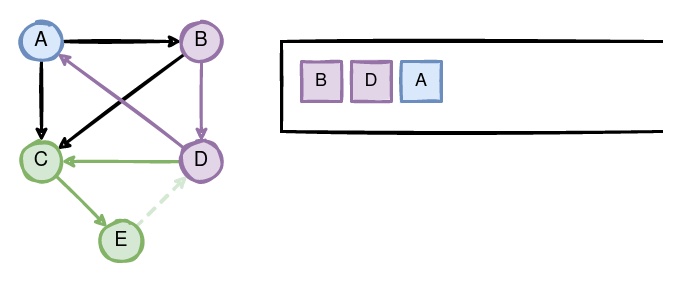
\includegraphics[width=0.8\linewidth]{images/graphs/graph-dfs-directed-10}
\end{center}
\end{frame}

\begin{frame}[fragile]
 \frametitle{Depth-first Search (DFS) dirigido}\small
\begin{center}
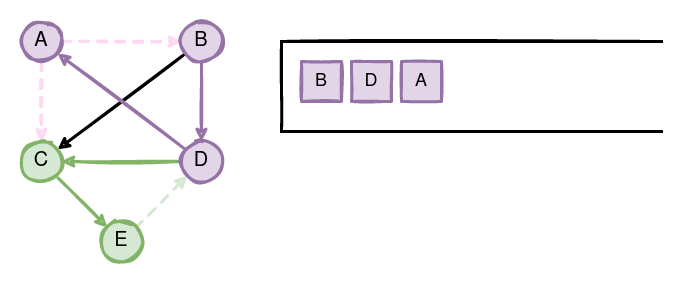
\includegraphics[width=0.8\linewidth]{images/graphs/graph-dfs-directed-11}
\end{center}
\end{frame}

\begin{frame}[fragile]
 \frametitle{Depth-first Search (DFS) dirigido}\small
\begin{center}
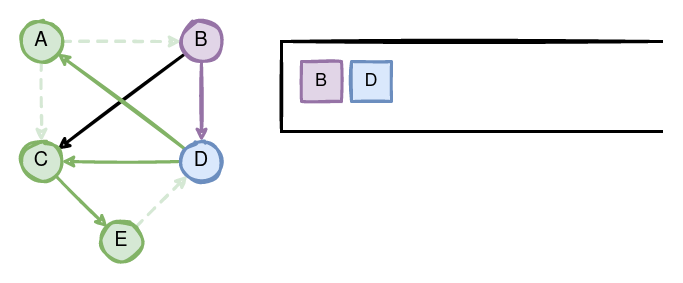
\includegraphics[width=0.8\linewidth]{images/graphs/graph-dfs-directed-12}
\end{center}
\end{frame}

\begin{frame}[fragile]
 \frametitle{Depth-first Search (DFS) dirigido}\small
\begin{center}
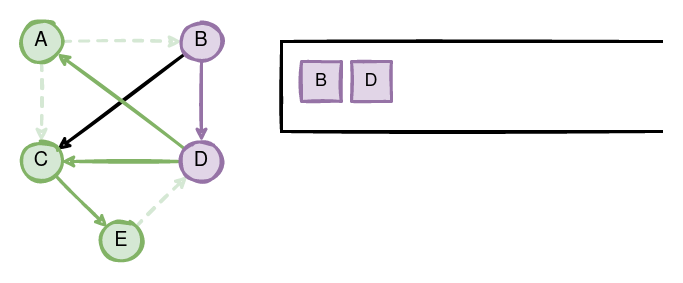
\includegraphics[width=0.8\linewidth]{images/graphs/graph-dfs-directed-13}
\end{center}
\end{frame}

\begin{frame}[fragile]
 \frametitle{Depth-first Search (DFS) dirigido}\small
\begin{center}
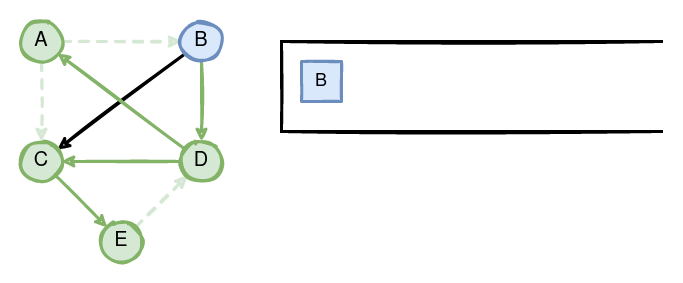
\includegraphics[width=0.8\linewidth]{images/graphs/graph-dfs-directed-14}
\end{center}
\end{frame}

\begin{frame}[fragile]
 \frametitle{Depth-first Search (DFS) dirigido}\small
\begin{center}
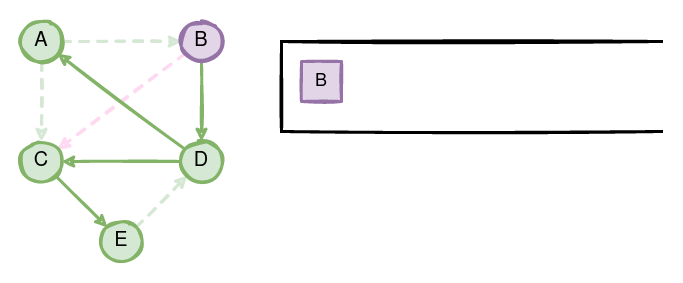
\includegraphics[width=0.8\linewidth]{images/graphs/graph-dfs-directed-15}
\end{center}
\end{frame}

\begin{frame}[fragile]
 \frametitle{Depth-first Search (DFS) dirigido}\small
\begin{center}
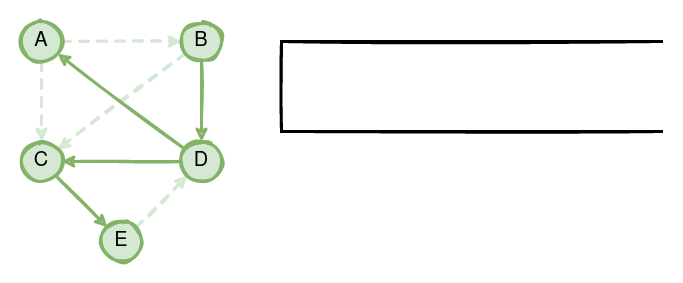
\includegraphics[width=0.8\linewidth]{images/graphs/graph-dfs-directed-16}
\end{center}
\end{frame}

\begin{frame}[fragile]
 \frametitle{Depth-first Search (DFS) Árbol Binario}\small
\begin{center}
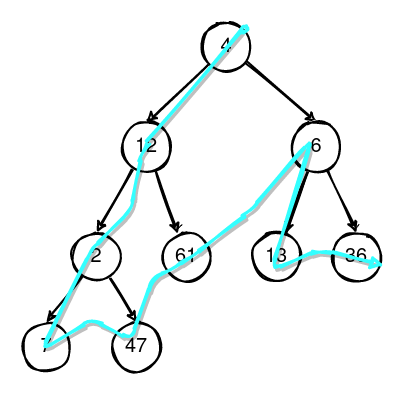
\includegraphics[width=0.8\linewidth]{images/dfs1}
\end{center}
\end{frame}

\begin{frame}[fragile]
 \frametitle{DFS: Ordenamiento Topológico}\small
\begin{itemize}
\item Un ordenamiento topológico es un ordenamiento lineal de tdos los vértices en un Grafo Drigido Acícliclo.
\item Si $G=(\mathcal{V},\mathcal{A})$ contiene un enlace $(x, y) \in \mathcal{A}$, entonces $x$ aparece antes que $y$ en el orden final.
\item Esto no sería posible si el grafo contiene algún ciclo.
\item Podemos ver un ordenamiento topológico de un grafo como un ordenamiento de sus vértices a lo largo de una línea horizontal, de modo que todos los enlaces dirigidos vayan de izquierda a derecha.
\item DFS es un algoritmo comunmente usado para esta labor.
\end{itemize}
\end{frame}

\begin{frame}[fragile]
 \frametitle{DFS: Ordenamiento Topológico}\small
\begin{center}
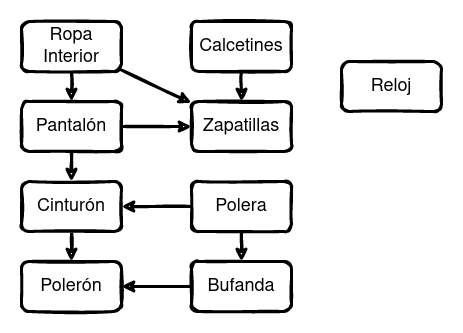
\includegraphics[width=0.8\linewidth]{images/graphs/graph-topsort-1}
\end{center}
\end{frame}

\begin{frame}[fragile]
 \frametitle{DFS: Ordenamiento Topológico}\small
\begin{center}
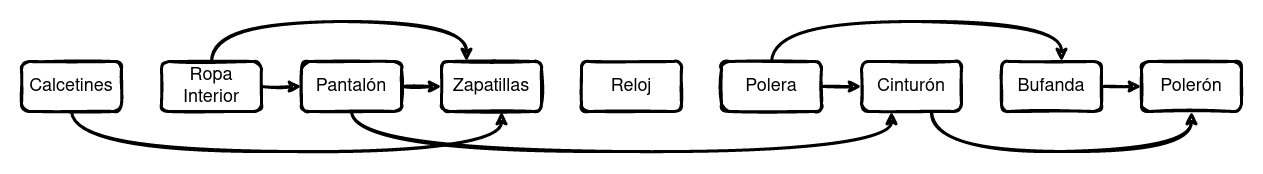
\includegraphics[width=0.8\linewidth]{images/graphs/graph-topsort-2}
\end{center}
\end{frame}


\begin{frame}[fragile]
 \frametitle{Ejercicios}
\begin{itemize}
\item Dar una representación de lista de adyacencia para un árbol binario completo de 7 vértices. Dar también una representación de una matriz de adyacencia para el mismo árbol. Asumir que los vértices están enumerados de 1 a 7.
\item Realice el recorrido BFS y DFS del siguiente grafo:
\begin{center}
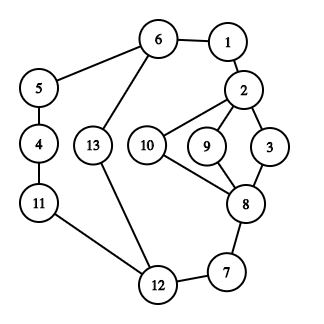
\includegraphics[width=0.5\linewidth]{images/graphs/example}
\end{center}
\end{itemize}
\end{frame}

\begin{frame}[fragile]
 \frametitle{Ejercicios}
\begin{itemize}
\item Realice el ordenamiento topológico del siguiente grafo: 
\begin{center}
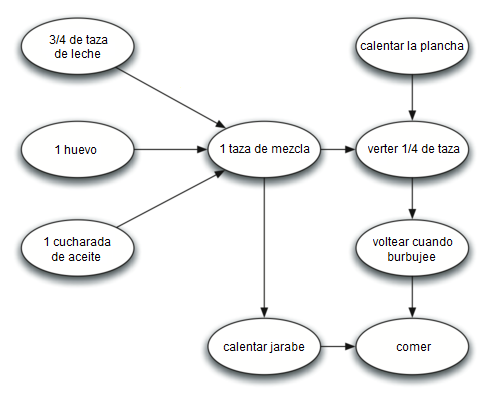
\includegraphics[width=0.5\linewidth]{images/graphs/pancakes}
\end{center}
\end{itemize}
\end{frame}



\end{document}
